\lstset{language={Python2}}

\title{ALPSチュートリアル: Introduction to Matplotlib}

\begin{document}

\begin{frame}
  \titlepage
\end{frame}

\section*{Outline}
\begin{frame}
  \tableofcontents
\end{frame}

\section{環境設定}
\begin{frame}[t,fragile]
\frametitle{デフォルトの環境設定}
図の中で使われる文字のサイズや,図の縦・横のサイズなどをあらかじめ設定しておくことができます.
\begin{itemize}
\item matplotlib \$\{HOME\}/.matplotlib/matplotlibrc で設定する
\begin{itemize}
\item テンプレを \$PYTHONHOME/lib/site-packages/matplotlib/mpl-data/matplotlibrc からコピーして使う
%% /opt/local//Library/Frameworks/Python.framework/Versions/2.7/lib/python2.7/site-packages/matplotlib/mpl-data/matplotlibrc
\item プロット時にウィンドウを開いて図を表示するには,Mac OS X の場合は次のような設定が必要
  \begin{lstlisting}
#backend : Agg
backend : MacOSX
\end{lstlisting}
\item 逆にウィンドウを開きたくないなら Agg に設定する
\item AGG: Anti-Grain Geometry. ベクトルデータを画像に描くライブラリ.C++ 用.
\end{itemize}
\end{itemize}

\end{frame}

\begin{frame}[t,fragile]
\frametitle{動的に環境設定を行う}
\begin{itemize}
\item backend の設定は import matplotlib の直後にすること
      \begin{lstlisting}
>>> import matplotlib as mpl
>>> mpl.use('Agg')
\end{lstlisting}
\item グラフのサイズやフォントのサイズの設定
      \begin{lstlisting}
>>> import pylab
>>> params = {
...     'legend.fontsize': 10
...     'xtick.labelsize':  8
...     'ytick.labelsize':  8
...     'figure.figsize':  [width, height]}
>>> pyalps.rcParams.update(params)
\end{lstlisting}
\end{itemize}
\end{frame}

\section{プロットしてみる}
\begin{frame}[t,fragile]
\frametitle{簡単な図をプロットしてみる}
\begin{columns}
\begin{column}{6cm}
$y = x^2$ のプロット
\begin{lstlisting}
>>> x = range(-10,10)
>>> y = [i*i for i in x]
# シンボルの色を赤(r),
# 形を丸(o)に設定
>>> pl.plot(x, y, 'ro')
...[<matplotlib.lines.Line2D at 0x114c82710>]
# 拡張子で保存の
# ファイル形式が決まります!
>>> pl.savefig('x2.pdf') 
>>> pl.show()
\end{lstlisting}
\end{column}

\begin{column}{6cm}
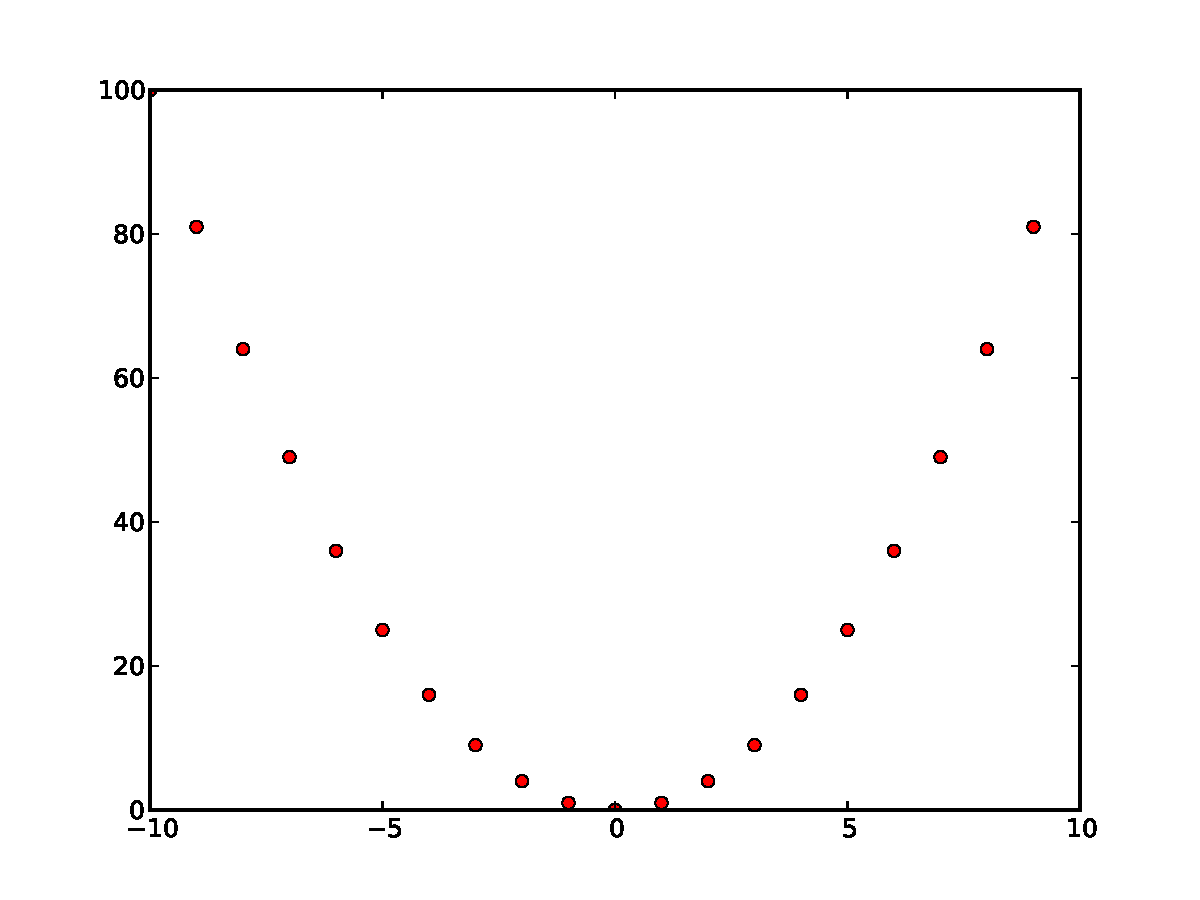
\includegraphics[width=\textwidth]{x2.pdf}
\end{column}
\end{columns}
\end{frame}

\begin{frame}[t,fragile]
\frametitle{少し複雑な図をプロットしてみる}
\begin{lstlisting}
>>> import math as m       # cos を使うため
>>> x = range(-10,10)
>>> y1 = [i*i for i in x]
>>> y2 = [i*i*i for i in x]
>>> y3 = [m.cos(2 * m.pi * i/20) for i in x]
# 図を上下 2 段に並べてプロットします
>>> pl.subplot(211)        # 上側の図を書き始めます
>>> pl.plot(x, y1, 'ro')   # 1 つのグラフに
>>> pl.plot(x, y2, 'b^')   # 2 つのデータセットをプロット
>>> pl.title('$x^2$ and $x^3$')   # 図のタイトル.TeX も Ok!
>>> pl.legend(('$y1$', '$y2$'), numpoints=1)  # 凡例
\end{lstlisting}
\end{frame}

\begin{frame}[t,fragile]
\frametitle{続き}
\begin{columns}
\begin{column}{6cm}
\begin{lstlisting}
# 下側の図を書き始めます
>>> pl.subplot(212)        
>>> pl.plot(x, y3, 'gs')
>>> pl.title('$\cos(x)$')
>>> pl.xlabel('x')
>>> pl.ylabel('y')
>>> pl.savefig('x3.pdf') 
>>> pl.show()
\end{lstlisting}
\end{column}
\begin{column}{6cm}
出来上がり!
\begin{center}
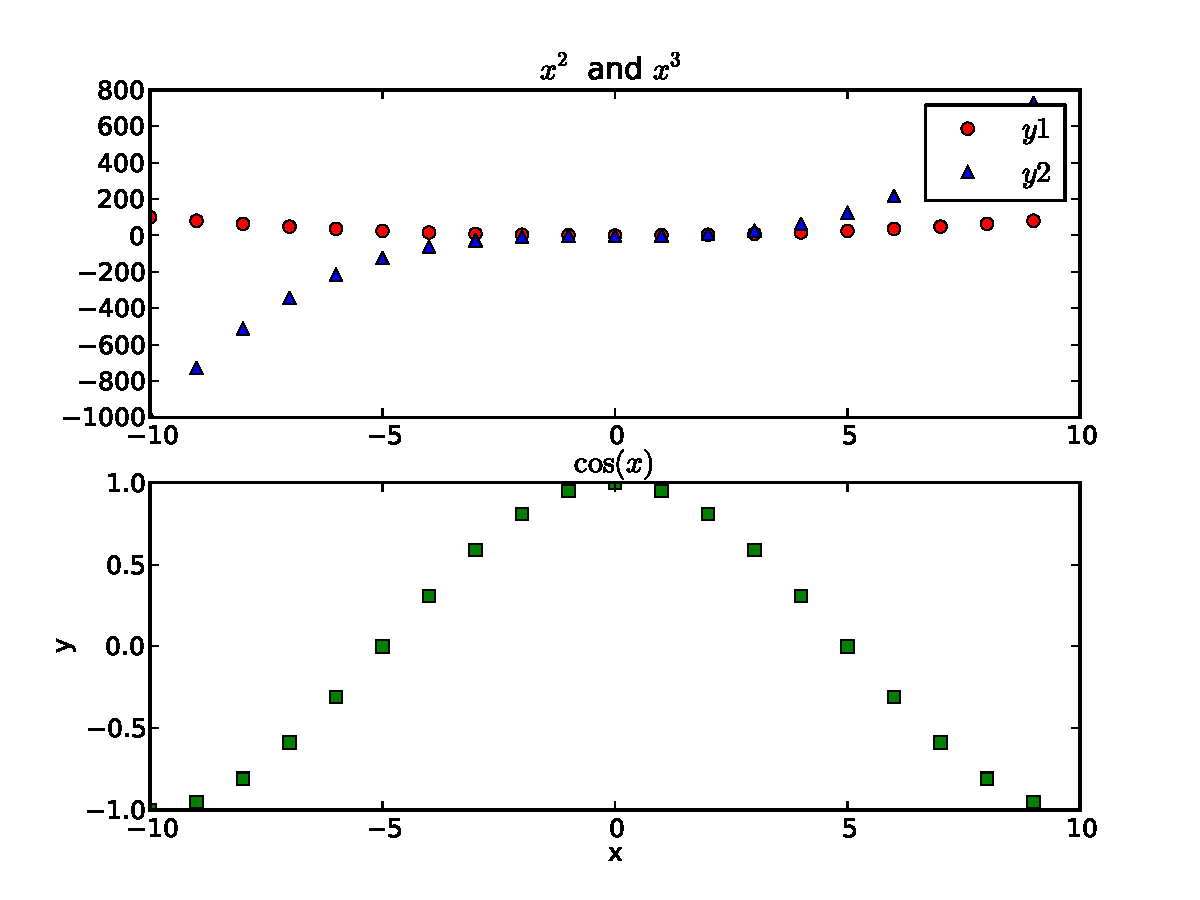
\includegraphics[width=\textwidth]{x3.pdf}
\end{center}
\end{column}
\end{columns}
\end{frame}

\section{Figure と Axes}
\begin{frame}[t,fragile]
\frametitle{Figure と Axes}
Matplotlib の描画領域には 2 つの座標系があります.
Figure と Axes です.1 つの Figure は 1枚の紙で,そこに複数のグラフ (Axes) を描くというイメージです.

Subplot は Axes の特殊なものです.subplot(col,row,pos) で描画位置を指定できます.

\begin{center}
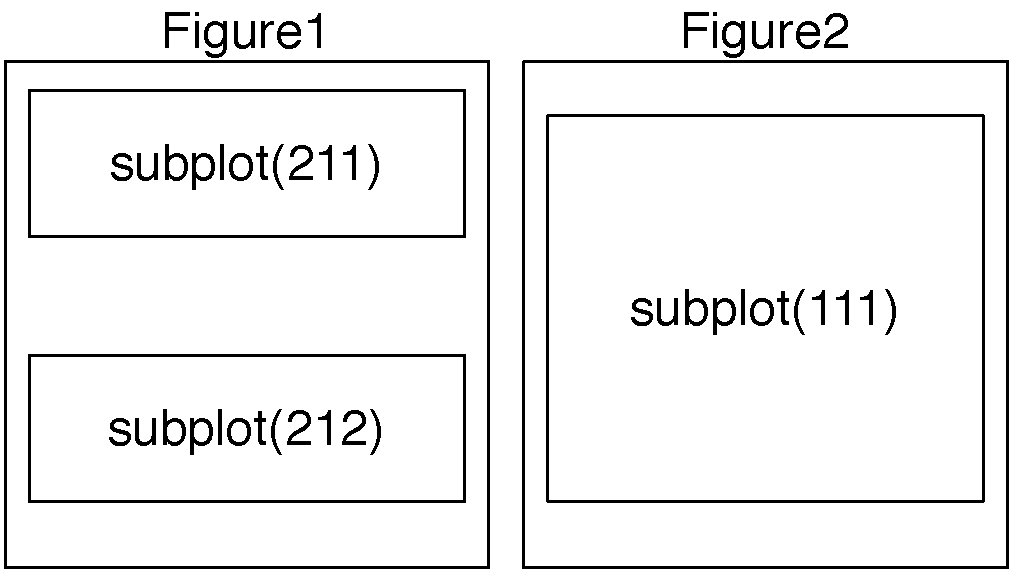
\includegraphics[scale=0.4]{fig_ax.pdf}
\end{center}
\end{frame}

\begin{frame}[t,fragile]
\frametitle{Current Figure/Axes vs. オブジェクト指向}
今まで紹介してきたプロットは,暗黙のうちに Current Figure/Axes への操作を行っていました.複数の Figure を同時に扱いたい場合はオブジェクト指向的なプロット方法が便利です.

\begin{columns}
\begin{column}{7cm}
\begin{lstlisting}
import pylab as pl

pl.figure() 
pl.plot(pl.rand(1000), 'o')

pl.figure()
pl.plot(pl.rand(1000), '^')

pl.show()
\end{lstlisting}
\end{column}

\begin{column}{7cm}
\begin{lstlisting}
import pylab as pl
fig1 = pl.figure() 
fig2 = pl.figure()

ax1 = fig1.add_subplot(111)  
ax2 = fig2.add_subplot(111)  

ax1.plot(pl.rand(1000), 'o')
ax2.plot(pl.rand(1000), '^')

pl.show()
\end{lstlisting}
\end{column}
\end{columns}
\end{frame}
\end{document}
